\documentclass[12pt]{article}
\usepackage[margin=1in,footskip=0.25in]{geometry}
\usepackage{amsmath,amsfonts,array,hyperref,graphicx}
\usepackage[style=verbose-ibid]{biblatex}
\usepackage{indentfirst}
\usepackage[indent=20pt]{parskip}

\title{GPU Accelerated L-System for Botanical Structures}
\author{Eric Lee, CS 179 Project}
\date{May 7, 2026}
\bibliography{cite}

\begin{document}

\maketitle

\section{Background}
In 1968, Aristid Lindenmayer introduced L-systems\autocite{Prusinkiewicz1990} to model the growth and development of multicellular filamentous organisms, such as the growth of algae and the branching architecture of higher plants. Unlike sequential rewriting systems, L-systems apply production rules in parallel to every symbol at each timestep, mirroring biological cell division in which daughter cells mature simultaneously. This formalism captures self-similar morphogenesis, simple deterministic rules generate intricate filaments, branching structures, and fractal curves that closely resemble natural botanical forms.
 
Beyond biology, L-systems generalize to classical space-filling fractals such as the Koch curve and Sierpi\'nski triangle. They also extend to bracketed alphabets\autocite{Ginsburg1967} that encode nested branching by pushing and popping a turtle's geometric state. Despite their simplicity, efficient evaluation is computationally demanding because string length grows exponentially with the iteration count, and bracketed structures introduce sequential dependencies making naive parallelization not possible.
 
\section{L-Systems}
Formally, an L-system is a triple $G = (V, \omega, P)$, where $V$ is a finite alphabet of symbols, $\omega \in V^+$ is the axiom (the initial string), and $P \subseteq V \times V^*$ is a set of production rules of the form $a \to \chi$, mapping each symbol to a replacement string. Starting from $\omega$, the system generates a sequence of strings $\sigma_0, \sigma_1, \sigma_2, \ldots$ by simultaneously rewriting every symbol of $\sigma_n$ according to $P$ to obtain $\sigma_{n+1}$. This simultaneous replacement is what distinguishes an L-system from a Chomsky grammar and is what makes derivation parallel.
 
To produce branching botanical forms, the alphabet is augmented with bracket symbols \texttt{[} and \texttt{]} that respectively push and pop the state of a turtle interpreter $(\mathbf{p}, \mathbf{R}) \in \mathbb{R}^3 \times SO(3)$. 

\noindent The standard turtle commands are:
\begin{itemize}
    \item \texttt{F}: move forward and draw a segment,
    \item \texttt{+}~/~\texttt{-}: rotate by a fixed angle $\delta$,
    \item \texttt{[}~/~\texttt{]}: push and pop the turtle state, beginning or ending a branch.
\end{itemize}
As a concrete example, consider the bracketed system for a fractal plant. The axiom is $\omega = \texttt{-X}$ and the production rules are
\begin{align*}
\texttt{X} &\to \texttt{F+[[X]-X]-F[-FX]+X}, \\
\texttt{F} &\to \texttt{FF},
\end{align*}
interpreted with rotation angle $\delta = 25^\circ$. Here, \texttt{X} does not correspond to any drawing action, it just controls the structural evolution of the curve. The first two derivations are:
\begin{align*}
\sigma_0 &: \texttt{-X}, \\
\sigma_1 &: \texttt{-F+[[X]-X]-F[-FX]+X}.
\end{align*}
Each \texttt{X} is replaced in parallel by the same branch-producing pattern wrapped with nested brackets, while every \texttt{F} simultaneously doubles. Consequently each iteration both lengthens existing segments and grafts new sub-branches throughout the structure. After only a few iterations, the turtle traces out a plant-like figure.
 
\begin{figure}[htbp]
    \centering
    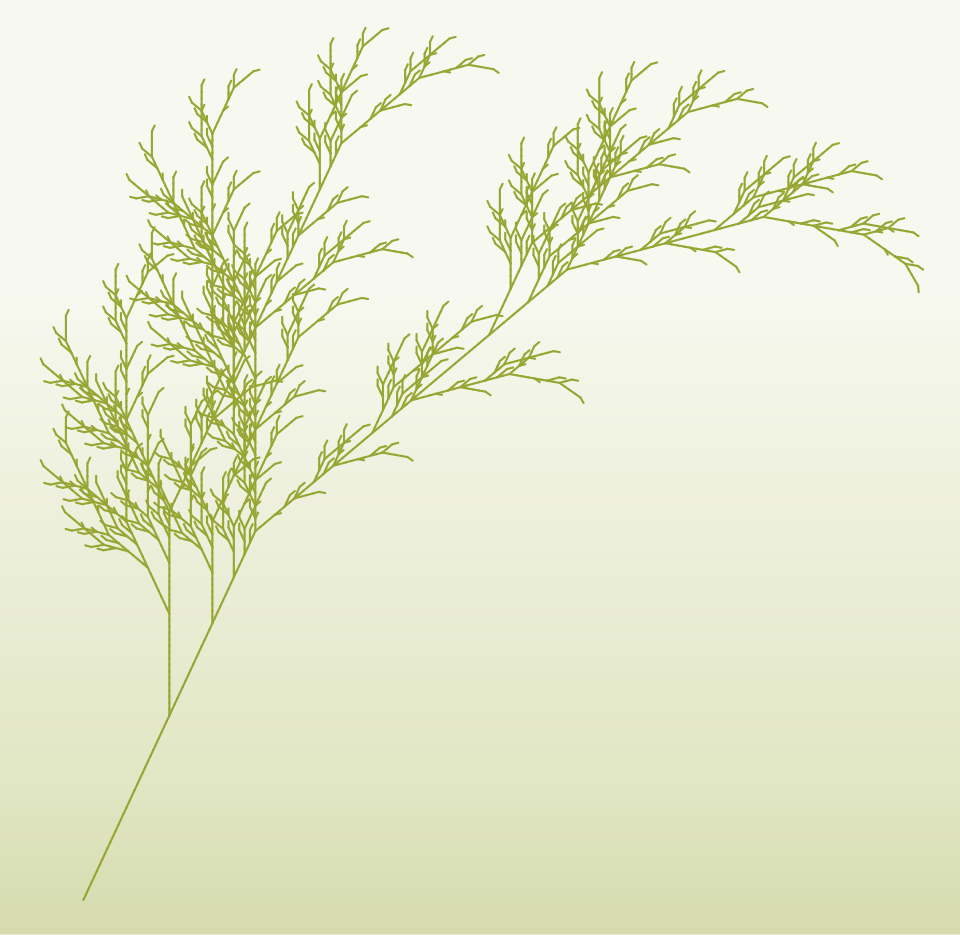
\includegraphics[width=0.4\textwidth]{../figs/fractal-fern.png}
    \caption{Barnsley Fern, $\sigma = 6$}
\end{figure}
 
The string length grows exponentially in the iteration count (here, $3^n$ symbols after $n$ rewrites of an \texttt{F}-only axiom under this rule), which is exactly what makes evaluation expensive on a CPU and attractive on a GPU.
 
\newpage
\section{Parallel GPU Algorithm}
We propose a hybrid CPU--GPU pipeline. The CPU parses the grammar, sequences iterations, and provides a sequential fallback for the bracketed branch-resolution stage. The GPU performs bulk string expansion, accumulates affine transforms through a parallel prefix scan, and writes geometry directly into OpenGL VBOs through CUDA. A sequential CPU implementation provides the correctness baseline and CPU timing data.

The primary issue is the variable-length. expansion of symbols. A single \texttt{F} may rewrite to many commands, and every symbol is replaced simultaneously, so threads cannot serially append to a shared buffer. We decompose one rewrite step into three phases:
\begin{enumerate}
    \item A length kernel assigns one thread per input symbol and records its production's output length in an array $L$.
    \item An exclusive prefix sum $S = \text{exclusive\_scan}(L)$ yields each thread's write offset.
    \item A scatter kernel writes the expanded tokens into the output buffer in parallel using offsets from $S$.
\end{enumerate}
Two preallocated ping-pong device buffers avoid repeated allocations, so iterating $n$ times produces $\sigma_n$ entirely on-device. For non-bracketed systems (Koch, Dragon, Sierpi\'nski), the world transform of the $i$-th segment is $T_i = \prod_{j=0}^{i-1} M_j$. Since matrix multiplication is associative, this reduces to a parallel exclusive scan over $4\times4$ affine matrices.

Bracketed systems introduce a dependency tree, as a branch must restore the transform stored at its matching \texttt{[}, which breaks the simple linear scan and rules out per-thread stacks (which would cause severe warp divergence and register pressure). Therefore, we adopt a hybrid strategy: the GPU still expands the string in parallel, but a lightweight CPU turtle interpreter resolves the brackets and writes vertices into the mapped VBO. This guarantees a working demo for fractal plants while still placing the asymptotically dominant work (string expansion, which grows exponentially) on the GPU.

Rendering will be doing through CUDA/OpenGL interop, where compute kernels write instance attributes (position, orientation, length, color) into a buffer that OpenGL consumes via instanced drawing, with orbit camera, anti-aliased lines, and optional bloom handled by the graphics pipeline.
 
\section{Deliverables and Goals}

The core work consists of a CPU proof-of-concept rewriter, a GPU string expander, a GPU transform engine that uses parallel matrix prefix scan for non-bracketed curves, and interactive OpenGL rasterizer with orbit camera with live parameter editing with the CUDA OpenGL interop. A performance pass will produce GPU and CPU speedup plots and Nsight Compute occupancy and bandwidth metrics.

There are some stretch goals if we finish early. First is a full GPU bracket reducer replacing the CPU interpreter via scan-based bracket matching and per-branch tree reduction. Another is CUDA Kawase bloom post-processing and other visualizations. Finally, it would be interesting to render fragment shaders in GLML (\url{https://www.glml-lang.com/}), a functional DSL compiling to GLSL written by the author to learn how to integrate a custom shader compiler with the CUDA/OpenGL pipeline.

\section{Proposed Timeline}
\begin{itemize}
    \item Week 1 (CPU baseline): Grammar parser, sequential rewriter, and turtle interpreter for both non-bracketed and bracketed systems, CPU timing data on various examples
    \item Week 2 (GPU string expansion): Kernels, validate against CPU output
    \item Week 3 (GPU rendering and CPU demo): Parallel matrix-scan for non-bracketed transform accumulation, OpenGL renderer with orbit camera, render fractal plant examples
    \item Week 4 (Profiling): Nsight Compute optimization, CPU vs. GPU comparisons, attempt the GPU bracket reducer if time permits, write-up
\end{itemize}

\hfuzz=30pt
\printbibliography
\end{document}
